\documentclass[dvipdfmx]{jsarticle}


\usepackage{tcolorbox}
\usepackage{color}
\usepackage{listings, plistings}

%% ノート/latexメモ
%% http://pepper.is.sci.toho-u.ac.jp/pepper/index.php?%A5%CE%A1%BC%A5%C8%2Flatex%A5%E1%A5%E2

% Java
\lstset{% 
  frame=single,
  backgroundcolor={\color[gray]{.9}},
  stringstyle={\ttfamily \color[rgb]{0,0,1}},
  commentstyle={\itshape \color[cmyk]{1,0,1,0}},
  identifierstyle={\ttfamily}, 
  keywordstyle={\ttfamily \color[cmyk]{0,1,0,0}},
  basicstyle={\ttfamily},
  breaklines=true,
  xleftmargin=0zw,
  xrightmargin=0zw,
  framerule=.2pt,
  columns=[l]{fullflexible},
  numbers=left,
  stepnumber=1,
  numberstyle={\scriptsize},
  numbersep=1em,
  language={Java},
  lineskip=-0.5zw,
  morecomment={[s][{\color[cmyk]{1,0,0,0}}]{/**}{*/}},
  keepspaces=true,         % 空白の連続をそのままで
  showstringspaces=false,  % 空白字をOFF
}
%\usepackage[dvipdfmx]{graphicx}
\usepackage{url}
\usepackage[dvipdfmx]{hyperref}
\usepackage{amsmath, amssymb}
\usepackage{itembkbx}
\usepackage{eclbkbox}	% required for `\breakbox' (yatex added)
\usepackage{enumerate}
\fboxrule=0.5pt
\parindent=1em
\begin{document}

%\anaumeと入力すると穴埋め解答欄が作れるようにしてる。\anaumesmallで小さめの穴埋めになる。
\newcounter{mycounter} % カウンターを作る
\setcounter{mycounter}{0} % カウンターを初期化
\newcommand{\anaume}[1][]{\refstepcounter{mycounter}{#1}{\boxed{\phantom{aa}\themycounter \phantom{aa}}}} %穴埋め問題の空欄作ってる。
\newcommand{\anaumesmall}[1][]{\refstepcounter{mycounter}{#1}{\boxed{\tiny{\phantom{a}\themycounter \phantom{a}}}}}%小さい版作ってる。色々改造できる。

%% 修正時刻: Tue May  5 10:19:29 2020


\section{TeraTermのインストール}

\subsection{TeraTermのダウンロード}

Google検索「teraterm」とすると、以下のサイトが一番上にくるはず。

\vspace{3mm}
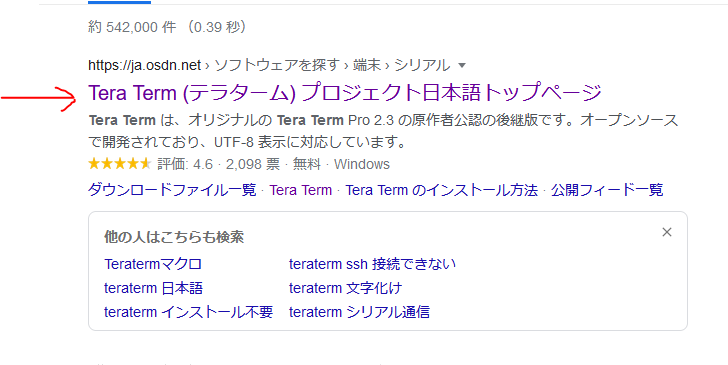
\includegraphics[width=12cm]{../img/01-teraterm-google.png}
\vspace{3mm}

このリンクをクリックすると、以下のページになる。

\vspace{3mm}
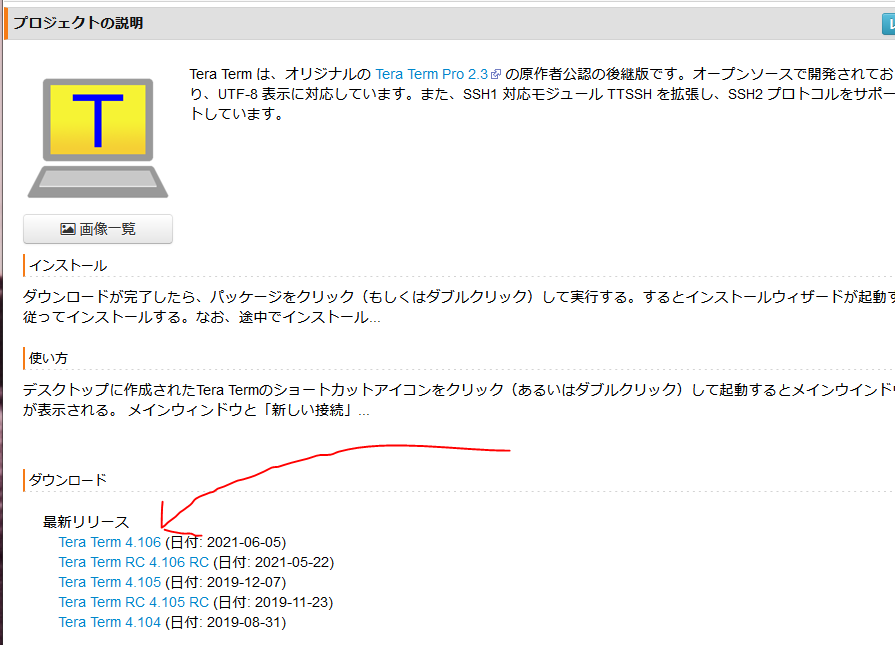
\includegraphics[width=12cm]{../img/02-teraterm-home.png}
\vspace{3mm}

''ダウンロード''の項目の''最新リリース''から、\textsf{Tera Term 4.106} をクリック。

\newpage
次に開いたページで、\textsf{teraterm-4.106.exe} と \textsf{teraterm-4.106.zip} の2つが
選択できるが、どちらも内容は同じ。
ここでは、\textsf{teraterm-4.106.exe} を選択する。

\vspace{3mm}
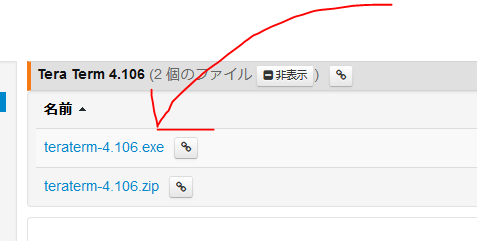
\includegraphics[width=10cm]{../img/03-teraterm-exe.png}
\vspace{3mm}

次のダイアログが表示されるので、''ファイルを保存''とする。

\vspace{3mm}
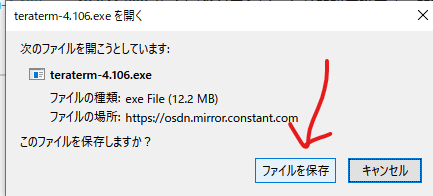
\includegraphics[width=10cm]{../img/04-teraterm-save.png}
\vspace{3mm}

すぐに保存される。ダウンロードフォルダに保存されるので、ダウンロードフォルダを開く。

\vspace{3mm}
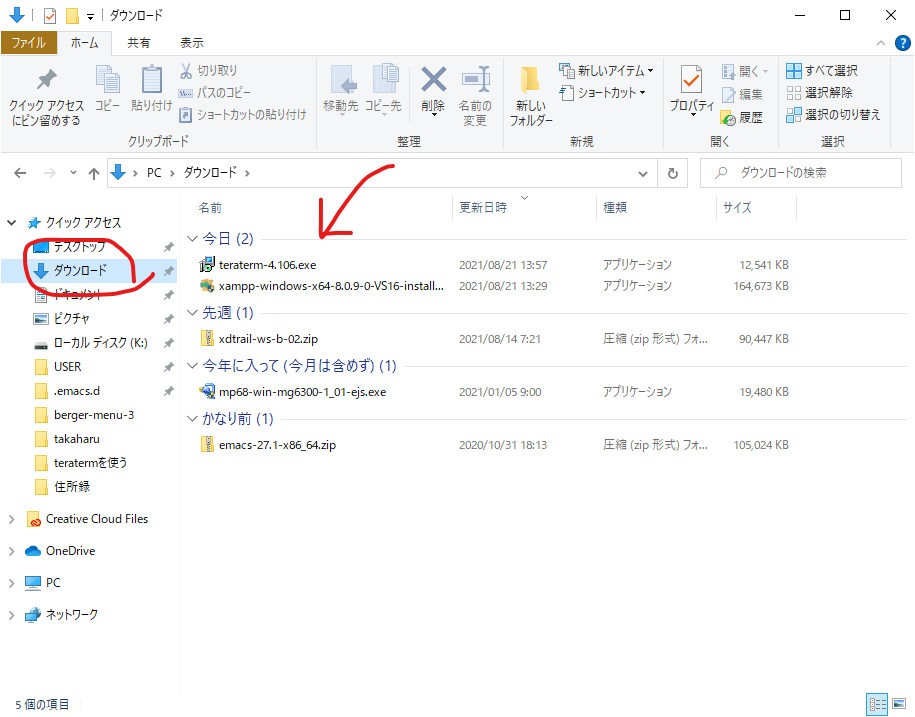
\includegraphics[width=11cm]{../img/05-download.png}
\vspace{3mm}

ダウンロードされた \textsf{teraterm-4.106.exe} をダブルクリックして、インストールを
始める。

インストールする言語に「日本語」を選択。

\vspace{3mm}
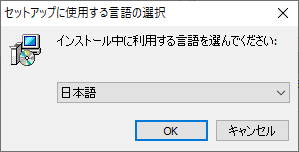
\includegraphics{../img/06-install-lang.png}
\vspace{3mm}

「使用許諾契約書の同意」は「同意する」にチェック。

\vspace{3mm}
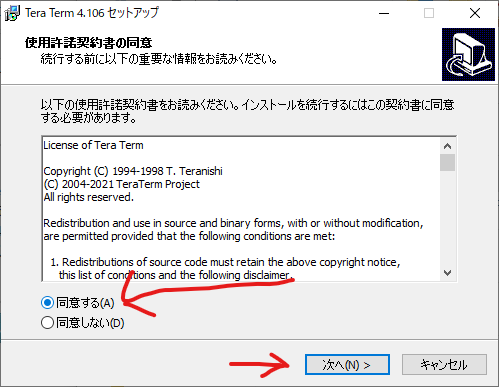
\includegraphics[width=10cm]{../img/07-agree.png}
\vspace{3mm}

\newpage
インストール先を確認。(\verb!C:\Program Files (x86)\teraterm!)

\vspace{3mm}
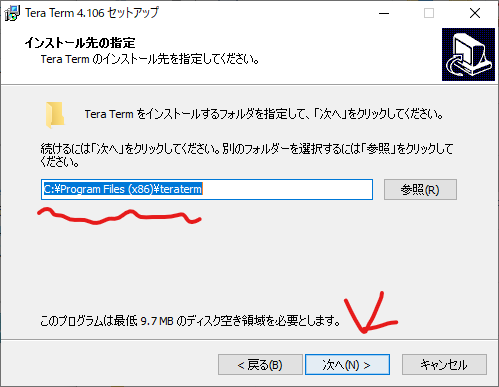
\includegraphics[width=10cm]{../img/08-install-folder.png}
\vspace{3mm}

次のコンポーネントの選択では、初期値のままでいく。

\vspace{3mm}
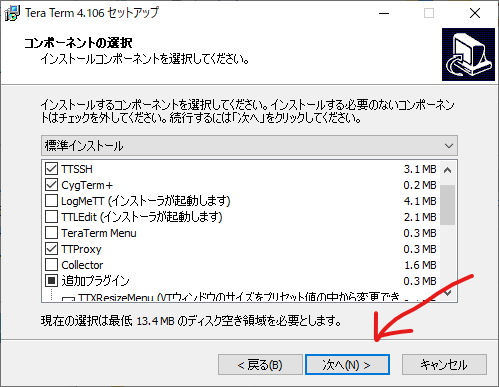
\includegraphics[width=10cm]{../img/09-select.png}
\vspace{3mm}

\newpage
言語の選択では、``日本語''を選択。

\vspace{3mm}
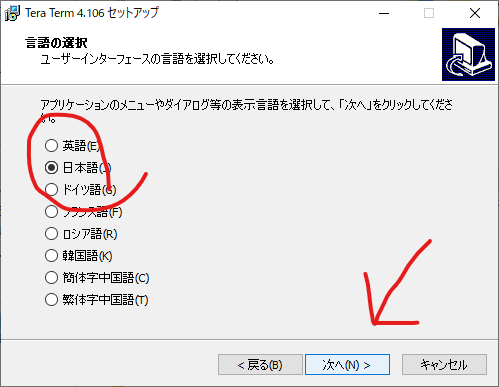
\includegraphics[width=10cm]{../img/10-select-jp.png}
\vspace{3mm}

プログラムグループの指定は、そのままで。

\vspace{3mm}
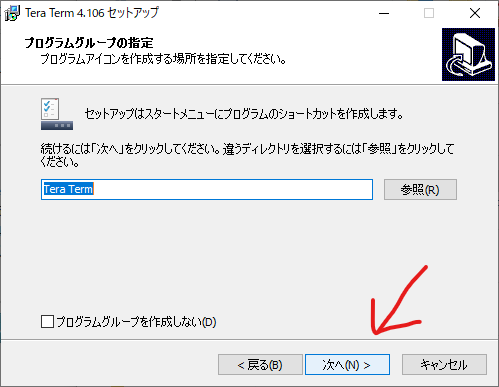
\includegraphics[width=10cm]{../img/11-next.png}
\vspace{3mm}

\newpage
追加タスクの選択も、そのままでクリック。

\vspace{3mm}
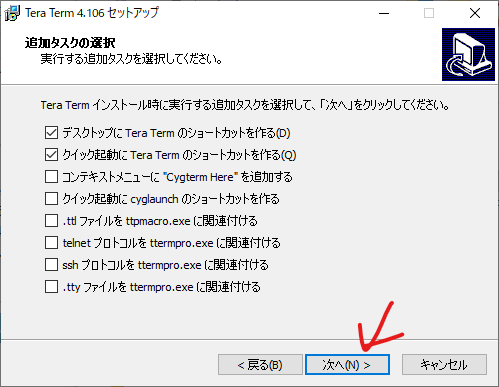
\includegraphics[width=10cm]{../img/12-relative.png}
\vspace{3mm}

確認画面。

\vspace{3mm}
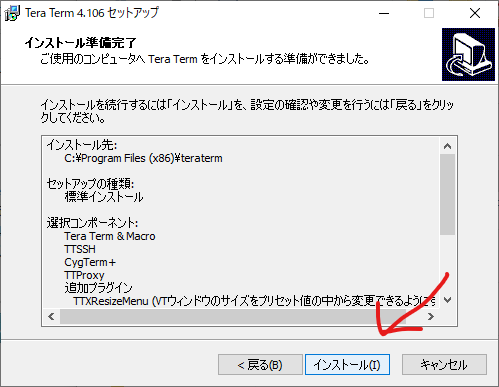
\includegraphics[width=10cm]{../img/13-last.png}
\vspace{3mm}

\newpage
完了。

\vspace{3mm}
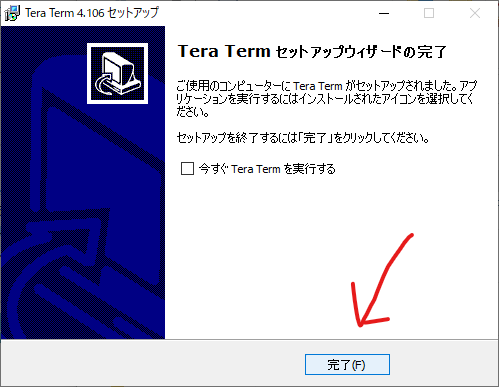
\includegraphics[width=10cm]{../img/14-install-end.png}
\vspace{3mm}







\end{document}

%% 修正時刻: Sat May  2 15:10:04 2020


%% 修正時刻: Sat Aug 21 18:28:38 2021
